\subsection{Baseline \& Replica}\label{sec:baseline_replica}
For analyzing Martian geological samples, the \gls{chemcam} team currently uses the \gls{moc} model~\cite{cleggRecalibrationMarsScience2017}.
This model integrates \gls{pls} and \gls{ica} to predict the composition of major oxides.

As shown in figure \ref{fig:moc_pipeline}, the input to the \gls{moc} model is the \gls{ccs} data, mentioned in Section~\ref{sec:problem_definition}.
This spectral data is collected on Earth in a laboratory setting simulating the Martian environment.
The instrument used to collect this data is a \gls{libs} instrument replicating the \gls{chemcam} instrument on the Curiosity rover.
Both the \gls{chemcam} and laboratory instrument consist of three spectrometers, each producing 2048 channels.
These spectrometers are used to capture the \gls{uv}, \gls{vio}, and \gls{vnir} regions of the spectrum.
For each sample, five \gls{ccs} datasets are collected by firing 50 laser shots at five different locations on the sample and processing the raw spectral readings \cite{wiensPreflightCalibrationInitial2013}.
Consequently, the \gls{ccs} data for each sample forms a high-dimensional Intensity Tensor $I$\ref{matrix:intensity} with dimensions $5 \times 50 \times 6144$.
An entry in this matrix represents the intensity of a specific wavelength in nanometers.
Complementing the data is the matrix of the corresponding major oxide concentrations for each sample $C$\ref{matrix:concentration}, which serves as the target variable for the model.
For more details, refer to Section 5 in \citet{p9_paper}.

The \gls{pls} and \gls{ica} phases of the \gls{moc} operate in parallel, and their predictions are blended to form the final predictions.
Though the \gls{moc} model has proven useful, it suffers from limitations in predictive accuracy and robustness.
An overview of the \gls{moc} model is shown in Figure~\ref{fig:moc_pipeline}.

\begin{figure}
	\centering
	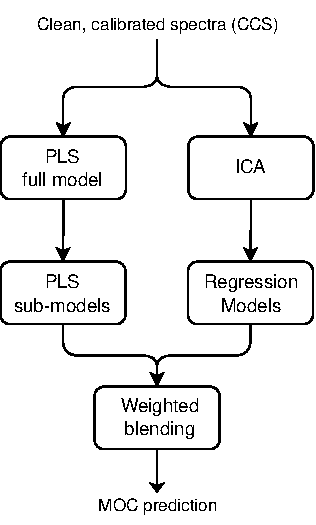
\includegraphics[width=0.225\textwidth]{images/moc_pipeline.pdf}
	\caption{Overview of the \gls{moc} model.}
	\label{fig:moc_pipeline}
\end{figure}

In \citet{p9_paper}, we presented our efforts to replicate the \gls{moc} model.
Based on the insights gained from that work, we have made several modifications to the replica in preparation for this work.

Our replica only utilized a single dataset for the \gls{ica} phase, while the original model used all five datasets.
This difference was due to the original paper not specifying how the five datasets were used, and so we designed an experiment to determine how to use them in a way that would most closely replicate the original model.
We initially assumed that the datasets were aggregated and used as a single dataset.
This approach, however, did not align with the original model's results, likely due to the loss of information from the individual datasets.
Following this discovery, we modified the replica to instead use the datasets in the same way as in the \gls{pls1-sm} phase, which yielded results aligning more closely with the original model.

Furthermore, our initial replica used a random train/test split for training, in contrast to the original model's manual curation to ensure representation of extreme compositions in both sets.
This difference stemmed from the original authors' application of domain expertize in their dataset curation --- a process we could not directly replicate.
Nevertheless, we found that automatically identifying extreme compositions and ensuring that they were present in both the training and testing sets brought us closer to the original model.
We chose to pull out the $n$ largest and smallest samples by concentration range, for each oxide, and reserve them for the training set.
Then we would do a random split on the remaining dataset, such that the final train/test split would be a $80\%/20\%$ split.

With these changes, we created a more accurate replica of the \gls{moc} model, which we will use as our baseline for the rest of this paper.
We have presented these changes to one of the original authors of~\citet{cleggRecalibrationMarsScience2017}, who confirmed that they were reasonable and in line with the original model's implementation.

Table~\ref{tab:replica_results_rmses} shows the \gls{rmse}s of the original models and our replicas after the changes.
Figure~\ref{fig:rmse_histograms} illustrates the distribution of these \gls{rmse}s as a grouped histogram.
The results show that the \gls{rmse}s of our replicas exhibit similar tendencies to the original models.
However, in some cases, our replicas have a lower \gls{rmse} than the original models, and in others, they have a higher \gls{rmse}.
These differences are due to a number of factors.

Firstly, the original models were trained with datasets from 1600mm and 3000mm standoff distances~\cite{cleggRecalibrationMarsScience2017}, while we only had access to the 1600mm dataset for our replicas.
Additionally, we automated the outlier removal for the PLS1-SM phase, unlike the original manual process.
As mentioned, the original authors manually curated their training and test sets, ensuring a broad elemental range, while we implemented an automatic process for our replicas due to lack of domain expertise.
Differences might also stem from varied implementation specifics, such as programming languages and libraries used.

\begin{table*}
	\centering
	\begin{tabular*}{\textwidth}{@{\extracolsep{\fill}}lllllll}
		\toprule
		Element    & \gls{pls1-sm} (original) & PLS1-SM (replica) & \gls{ica} (original) & ICA (replica) & \gls{moc} (original) & \gls{moc} (replica) \\
		\midrule
		\ce{SiO2}  & 4.33                     & 4.52              & 8.31                 & 8.63          & 5.30                 & 5.61                \\
		\ce{TiO2}  & 0.94                     & 0.49              & 1.44                 & 0.54          & 1.03                 & 0.61                \\
		\ce{Al2O3} & 2.85                     & 1.79              & 4.77                 & 3.18          & 3.47                 & 2.47                \\
		\ce{FeO_T} & 2.01                     & 2.16              & 5.17                 & 2.87          & 2.31                 & 1.82                \\
		\ce{MgO}   & 1.06                     & 0.91              & 4.08                 & 3.11          & 2.21                 & 1.56                \\
		\ce{CaO}   & 2.65                     & 1.73              & 3.07                 & 3.28          & 2.72                 & 2.09                \\
		\ce{Na2O}  & 0.62                     & 0.80              & 2.29                 & 1.39          & 0.62                 & 1.33                \\
		\ce{K2O}   & 0.72                     & 0.72              & 0.98                 & 1.38          & 0.82                 & 1.91                \\
		\bottomrule
	\end{tabular*}
	\caption{\gls{rmse}s of the original and our replicas of the \gls{pls1-sm}, \gls{ica}, and \gls{moc} models.}
	\label{tab:replica_results_rmses}
\end{table*}

\begin{figure*}
	\centering
	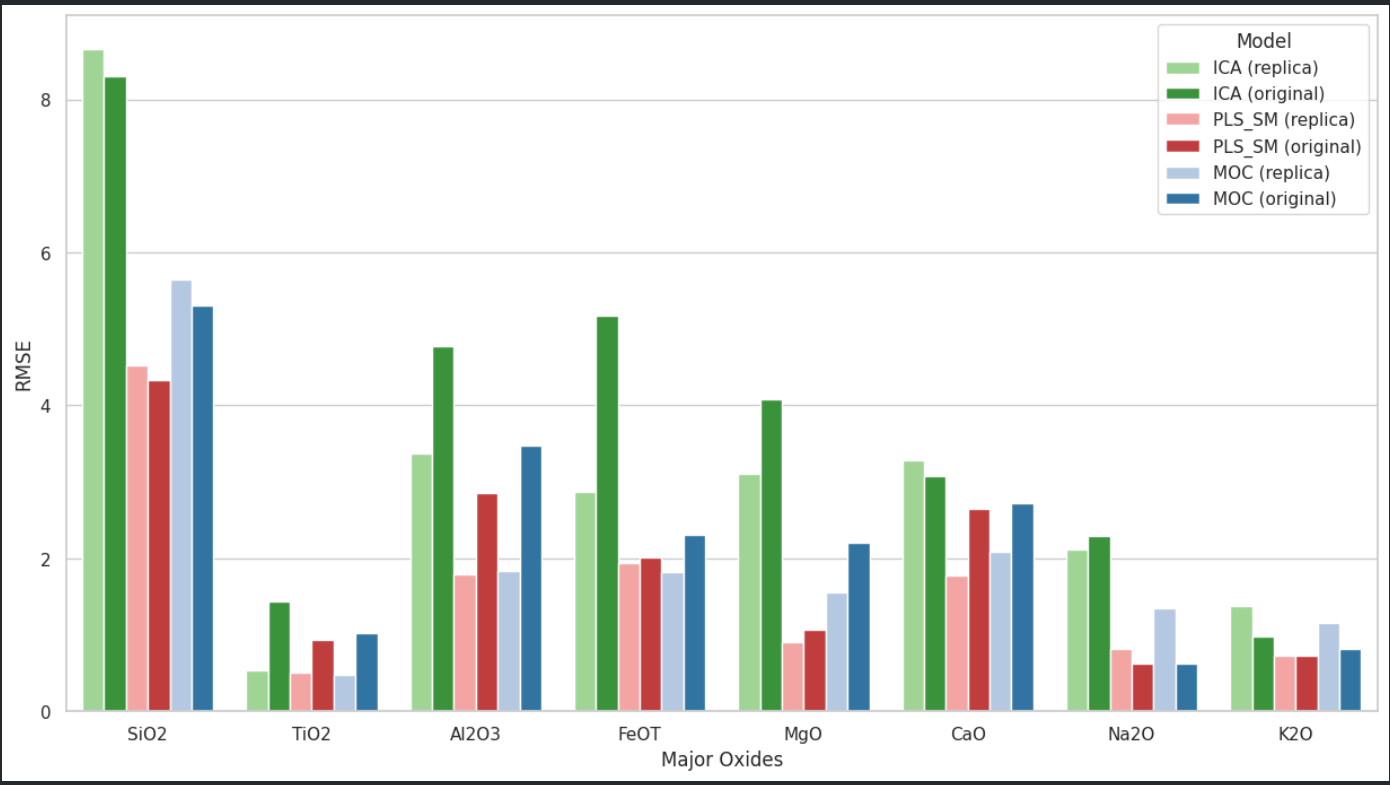
\includegraphics[width=0.85\textwidth]{images/rmse_historgram.png}
	\caption{Grouped histogram of the \gls{rmse}s of the original and our replicas of the \gls{pls1-sm}, \gls{ica}, and \gls{moc} models.}
	\label{fig:rmse_histograms}
\end{figure*}

Through a series of comparative experiments, we showed that the model selection was the primary cause of these limitations, and we showed how both \gls{ann} and \gls{gbr} methods could be used to improve the model's predictive accuracy and robustness.
This is further underscored by work from the SuperCam team.
In 2021, the Perseverance rover landed on Mars, equipped with the SuperCam instrument, which is the successor to the \gls{chemcam} instrument.
As part of the ongoing work to support the SuperCam instrument, \citet{andersonPostlandingMajorElement2022} experimented with various machine learning models to predict the composition of major oxides in geological samples using the SuperCam \gls{libs} calibration dataset.
While the team decided to retain \gls{pls} for analyzing certain oxides, \gls{ica} was entirely discontinued.
Instead, models based on \gls{gbr}, \gls{rf}, and \gls{lasso} were selected for other oxides.
This decision reinforces our finding that \gls{ica} regression models fall short in accurately predicting the composition of major oxides in geological samples.
Consistent with our observations, \gls{gbr} was also identified as a high-performing model in their analyses.
